\chapter{Statistical data in~the~context of~Linked Data}
\label{ch:statistical-data}
To understand the~rest of~the~thesis, let us~talk about the~aforementioned models.
We will take the~description step by~step, starting with a~dataset stored in~a~plaintext file.
After a~while, we~will get familiar with RDF, Linked Data and~last, but not least, with the
Data Cube Vocabulary.

Since we~are discussing statistical data, we~will use a~simple real--life example.
National statistical offices all over the~world are well--known for periodic gathering of~the
statistics about the~population of~the~country they are operating in. Moreover, 
those statistics are being regularly published and~gathered by~international 
organizations, e.g. the~UN~\cite{un} which can make a~comparison and~build 
another statistics upon the~national data. Also, other organizations, like 
Google~\cite{pubdata} use those data to~publish them and~make 
some advanced statistics.

That is, in~fact, why we~would like to~have the~data in~a~pre--defined structure,
wrapped with metadata to~perfectly understand what the~data in~a~given 
dataset mean. Moreover, we~would take advantage of~such a~dataset to~speed up~and~automate its processing. It~would be~great to~be~able to~introduce a~tool, 
which will take the~national statistics immediately after its publishing and~deliver a~new version of~the~international dataset without the~need of~any~user 
input.

\section{From speech to~structured data}

We will introduce the~reader to~the~problem by~examining an~example based on~the~total number of
citizens living in~the~country. That is~a~very simple kind of~information, but we~will demonstrate
how this could be~put into~the~context of~the~models mentioned in~the~introduction.

Let us~start with a~dataset with only one entry:

\begin{verbatim}
The Czech Republic has 10 505 445 citizens.
\end{verbatim}

That is~a~sentence a~normal person would say but it~holds a~statistical information.
If we~wanted to~keep this information in~a~simple structured text file, we~would e.g. name it
\texttt{number\_of\_citizens.txt} and~it~would have the~following contents:

\begin{verbatim}
Czech Republic     10505445
\end{verbatim}

Normally, we~keep this kind of~statistics to~make a~comparison, 
for instance, to~compare the~total number of~citizens of~all the~countries in~the~world.
We will, however, continue with just the~two of~them:

\begin{verbatim}
Czech Republic	    10505445
Slovakia	          5404555
\end{verbatim}

That gives us~a~dataset with two entries. Each entry is~consisted of~two parts. Let us~notice, that 
its semantics are kept in~the~reader's head. The~document itself does not keep the~information.
To process the~data, it~is~necessary to~know what the~information in~the~file represents. You could change
the~contents of~the~file into~the~following form:

\begin{verbatim}
Czech Republic      10505445
Slovakia            5404555
Meat                like
Fruit               orange
\end{verbatim}

Such a~dataset is~technically correct (values are separated by~tabulators), nevertheless 
semantically, it~makes no~sense. After reading the~contents of~the~file, the~reader 
is aware of~the~fact that in~the~given context the~added lines do~not fit in.
Let us~return to~the~meaningful example.

If we~keep the~meaning of~the~values, we~know that in~the~first column we~have the~name
of the~country and~in~the~second one, we~have the~total number of~citizens. Those statements
could be~called \emph{observations}, as~it~can be~said that~someone made an~observation 
about there being over 10 million people living in~the~Czech Republic. We~can also say that the
dataset has got two \emph{dimensions}. The~first one is~the~place where the~observation has taken
place, the~second one is~the~value being measured.

That would make a~nice Excel table, simple chart or~a~nice map of~central Europe with
two labels. Those are the~usual ways of~processing such datasets.

Now, let us~get back to~the~very first statement:

\begin{verbatim}
The Czech Republic has 10 505 445 citizens.
\end{verbatim}

\begin{sloppypar}
When transferring the~statement into~a~more technical form, we~forgot to~extract one
dimension. The~sentence also carries information about time. This is~quite an~important
part of~the~information since the~count of~citizens of~the~specific country evolves with time.
People are dying as~well as~getting born. Since the~sentence is~presented while using the
present tense, we~can conclude that~the~observation is~valid for the~current year (2013).
\end{sloppypar}

That means the~dataset stored in~a~plaintext file should look similar to~this:

\begin{verbatim}
Czech Republic       10505445     2013
Slovakia	            5404555      2013
\end{verbatim}

The last column evidently holds the~year of~the~observation being made.
That gives us~three dimensional dataset. We~know the~place, the~total number of~citizens and~the~time of~the~measured value being acquired.

Now, we~may come to~a~decision of~publishing such a~document to~the~Web. We~can transform
it into~a~web page and~publish it~on~a~server.
\begin{figure}
\small\begin{verbatim}
<html>
    <head>
        <title>Number of citizens in a country</title>
    </head>
    <body>
        <table>
            <thead>
                <tr>
                    <th>Country name</th>
                    <th>Number of citizens</th>
                    <th>Year</th>
                </tr>
            </thead>
            <tbody>
                <tr>
                    <td>Czech Republic</td>
                    <td>10505445</td>
                    <td>2013</td>
                </tr>
                <tr>
                    <td>Slovakia</td>
                    <td>5404555</td>
                    <td>2013</td>
                </tr>
            </tbody>
        </table>
    </body>
</html>
\end{verbatim}\normalsize
\caption{An example of~an~HTML file with tabular data}
\label{fig:rdf-html-01}
\end{figure}

Example of~such a~web page source code can be~seen in~Figure~\ref{fig:rdf-html-01}. We~published the~data not only in~a~more structured form but also
provided an~explanation of~its meaning. Therefore, some additional data had to~be~added. In~fact, we
should speak of~it~as~of~metadata, since the~meaning is~rather descriptive instead of~semantical.

With a~specifically programmed script or~a~tool (so-called \emph{scraper}) it~is~possible to
convert such a~web page into~another format or~make an~eye--catching visualization.
But one gets to~learn the~tool, the~meaning of~the~data, its structures and~the~handling of~each of~the~dimensions. Moreover, one is~not able to~gather more information,
because there is~not any~in~the~document itself and~there is~no~way of
automatically linking the~values in~the~document to~other documents (unless, of~course,
one is~developed).

This is~where the~Resource Description Framework~\cite{rdf} and~the~Linked Data~\cite{ld}
model come in. Those
can help us~introduce some semantical meaning to~link entities in~the~document to
other entities on~the~Internet. Let us~provide more details about the~RDF before getting
back to~this example.

\section{Resource Description Framework}
As stated before, the~Resource Description Framework is~one of~the~most used models for
describing data with metadata. Its purpose is~to~give a~common model for data interchange
on the~Internet in~order to~make all its users able to~exchange data with semantics.
It introduces a~way of~describing a~schema of~the~interchanged data. It~also 
offers features that help facing a~situation when two datasets describe the~same thing,
but have different schemas.

The standard model of~the~web works on~the~principle of~URIs. Each page, which is, in~fact,
an~entity or~resource, has a~URI, which stands for its unique identifier. Nothing on~the~web
should have the~same identifier. What RDF adds to~this model is~that even relations
between those resources have their URIs. An~example of~such a~relation could be:

\tiny\begin{verbatim}
http://dbpedia.org/resource/Kenya   http://www.w3.org/1999/02/22-rdf-syntax-ns#type http://dbpedia.org/ontology/Country  
\end{verbatim}\normalsize

This actually tells us~that \texttt{Kenya is~a~country}. That statement could obviously be~found on
the~Internet in~a~countless of~different data sources; they are not usually presented
in a~machine--readable form, though. In~order to~work with that sentence we~need a~parser, which is~able to~get the~information based on~a~bunch of~linguistical rules.
Moreso, the~sentence might be~more complicated, e.g. \texttt{Kenya, with Nairobi as~its capital city,
is a~very beautiful country}. Ignoring the~fact that the~sentence brings another useful
information, we~should aim our focus on~the~fact that it~is~more of~a~complicated piece of~language to~parse. 

The RDF notation gives a~semantic meaning to~the~relation. The~RDF model is~based on~making certain
kinds of~triples; such can be~seen in~the~previous example. If~we~extend the~set of~triples with another,
what we~get is~\emph{a directed labeled graph}, where an~edge represents \emph{relation} between two resources.
Those resources are represented by~graph nodes. Based on~the~actual content of~the~triples,
the~graph may consist of~two or~more standalone connected components as~well as~of
just a~single one. Such a~graph may potentially contain information about~entities from all over
the~Internet, which would be~very useful.

The main point is, that all the~information published with~respect to~the~RDF model may be
automatically processed by~a~computer able to~work with the~semantics without
needing the~user to~specify it~(as somebody has already done that while publishing the~dataset).

\section{Linked Data}

One implementation of~the~Resource Description Framework is~the~Linked Data model.
It utillizes several technologies and~principles to~actually interconnect the~data on~the~Internet.
Both resources and~relations are denoted with URIs. The~HTTP protocol is~used to~make
the~resource public on~the~Internet. It~may be~found by~dereferencing (accessing) the~assigned
URI. Both machines and~people are therefore capable of~looking the~resource up.

When the~URI is~dereferenced, more useful information could be~provided while utillizing the~RDF
and SPARQL standards. Since the~model is~called Linked Data, the~most significant part
of the~concept is~about knowing how the~data could be~connected when being published on~the~Web.
It also brings some serialization formats, such as~RDFa, RDF/XML, N3, Turtle and~many others.
One of~the~most significant projects involving Linked Data is~the~LOD2 project~\cite{lod2}
(its visualization can bee seen) in Figure~\ref{fig:lod-cloud}.

To make the~idea about datasets more clear, let us~mention some well--known data sources
involving Linked Data:

\begin{itemize}
\item DBPedia --- dataset made by~transforming Wikipedia into~the~RDF model.
\item FOAF --- dataset describing persons, their properties and~relationships.
\item GeoNames --- geographical LD~database.
\item CKAN --- community--run catalogue of~useful sets of~data on~the~Internet.
\end{itemize}

\subsubsection{Namespaces and~prefixes}

There is~one rather technical note we~should mention before taking further steps. The~RDF
also brings a~way of~expressing URI of~a~resource in~a~more compact form while utilizing
so--called prefixes and~namespaces. Let us~look at~an~example:

\scriptsize\begin{verbatim}
http://dbpedia.org/ontology/populationTotal
http://dbpedia.org/ontology/populationAsOf
\end{verbatim}\normalsize

Those are URIs which reference specific properties with a~semantic meaning as~designed
by the~DBPedia~\cite{dbpedia}. At~a~closer look, one can see that there are some parts of~the~URI
that are repeated in~each of~them. E.g. the~scheme --- http. Although that is~a~rather technical
point of~view. The~most long common part of~both URIs is~\url{http://dbpedia.org/ontology/}
which makes a~namespace. It~makes a~logical sense that all the~resources in~the~virtual
folder \texttt{ontology} have something in~common, therefore, they are grouped into~the~namespace.

\begin{sloppypar}
Since one could remember easily the~name of~the~specific resource in~a~namespace,
e.g. \texttt{populationTotal}, it~would be~great if~they had no~need to~look up~the~full
URI of~the~namespace and~express it~with a~short and~easy--to--remember, but still 
unique, identifier. That is~what prefixes are designed for. For instance, the
\url{http://dbpedia.org/ontology/} was assigned the~prefix \texttt{dbpedia-owl}. Since the~scheme
is then \texttt{prefix:localname}, one could write:
\end{sloppypar}

\scriptsize\begin{verbatim}
dbpedia-owl:populationTotal
dbpedia-owl:populationAsOf
\end{verbatim}\normalsize

which is~equivalent to~the~previous example. It~is~then a~lot easier to~write RDF
documents for a~human being, especially while using well--known prefixes. A~kind of~unofficial
registry could be~found on~\cite{prefixcc}.

In order to~get the~processes in~a~country more transparent, governments also publish data
related to~the~country (statistics, public spendings data, …) to~the~Internet. Not many of
them are published in~the~form of~the~Linked Data, so~there are many initiatives
interested in~transforming the~data into~a~machine-readable form.

It is~definitely a~great achievement to~have such a~dataset in~a~form of~Linked Data, but
what we~need for understanding its contents is~a~suitable visualization of~the~data.
Due to~our knowledge of~working with statistical multi--dimensional data we~can apply our know--how
to the~aforementioned data as~they are statistical datasets as~well.

\begin{figure}
	\centering
	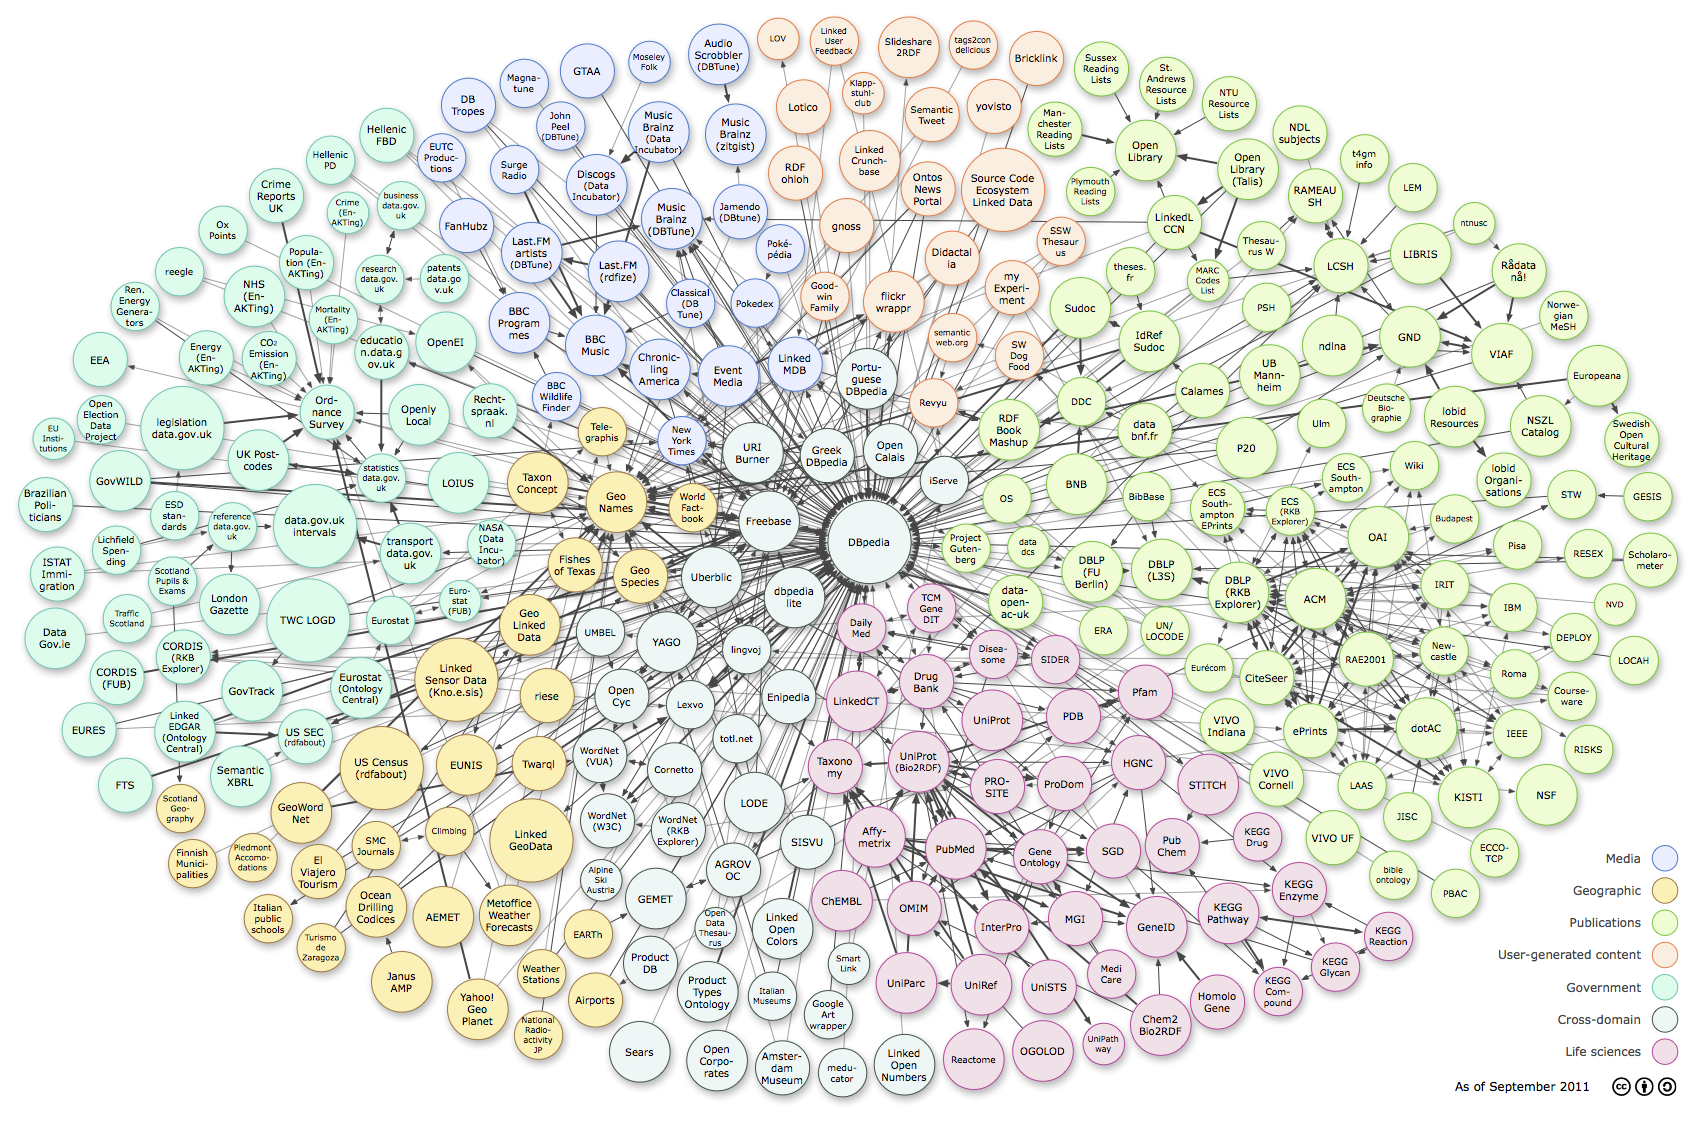
\includegraphics[width=150mm]{img/lod-cloud.png}
	\caption{LOD cloud diagram by~Anja Jentzsch~\cite{lod-cloud} (situation as~of~19. 9. 2011)}
	\label{fig:lod-cloud}
\end{figure}

Our aim is~to~have a~description model, which annotates a~dataset with a~semantically--specific
notation. That would enable us~to~generalize the~processes involving statistical Linked Data
and prepare some universal types of~visualizations, which are commonly used in~the~non-LD world.

\subsubsection{Ontologies}

Let us~also introduce the~concept of~an~ontology, which is~a~product of~the~RDF evolution.
The Resource Description Framework is~not very restrictive. One can build his own content
of a~RDF document, e.g.:

\scriptsize\begin{verbatim}
http://example.com/Czech_republic	http://example.com/relation/hasCapital	http://example.com/Prague
\end{verbatim}\normalsize

or

\scriptsize\begin{verbatim}
http://pedia.rdf/Czech_republic	http://pedia.rdf/hasCapital	http://pedia.rdf/Prague
http://pedia.rdf/Czech_republic	http://pedia.rdf/language	http://pedia.rf/Czech
\end{verbatim}\normalsize

By comparing the~first lines from each of~the~documents, it~might be~apparent they hold the~same
information; that the~capital city of~the~Czech Republic is~Prague. At~a~closer look, a~more observant
reader can notice, that each of~them uses different URIs to~dereference the~resources related to~the
Czech Republic and~Prague (in fact, they use different namespaces to~make the~reference).
They also use different URIs (and namespaces) to~express the~relation
between a~country and~its capital.

Moreso, the~second document holds more information as~it~tells us, that people of~the
Czech Republic speak Czech. Both documents are perfectly valid and~could be~published on~the~Web. That is~why the~concept of~ontologies was introduced.
With an~ontology, one may specify the~requested outline of~the~document.

When formalized as~defined in~\cite{ldvm2}:
\emph{An ontology $O$ is~a~triple $(C,P,M)$ where~$C$ is~a~set of~classes, $P$ is~a~set of
predicates and~$M$ is~a~set of~RDF statements (mappings of~the~classes and~properties to
other ontologies). Both classes and~predicates are specified using their unique URIs.}

Let us~start with countries. Without a~restriction, one may also include, let us~say, planets. With
an~ontology, it~can be~specified what kind of~resources could be~included.
It is~needed to~specify a~URI describing the~type \texttt{country}, for instance
a rule can be~set that a~resource needs to~be~of~the~type \mbox{\url{http://schema.org/Country}}.

After that, another rule is~added, which will define that the~country may have its capital
specified. Let us~say one decides to~go~with the~relation described by~dereferencing the~URI of
\texttt{dbpprop:capital}. 

It is~clear, that none of~the~examples conform, since neither of~them utilizes the~relation
\verb dbpprop:capital. This is~a~very simple example of~how ontologies could be~used. What we
did was that we~utilized the~possibility to~constraint properties of~a~resource.

\begin{sloppypar}
A new language, OWL (Web Ontology Language)~\cite{owl}, was developed based on~the~RDF in~order to
standardise the~way of~making restrictions. It~gives us~much stronger possibilities than just
restricting the~properties, which is, on~the~other side, the~most commonly used technique.
\end{sloppypar}

\subsubsection{Example with the~usage of~RDFa}

Now, let us~get back to~the~example related to~the~number of~citizens in~a~country. At~first, we
will alter the~HTML document to~involve some semantics. To~achieve that, we~will utilize the
RDFa model, as~can be~seen in~Figure~\ref{fig:example-rdfa}.

\begin{figure}
\scriptsize\begin{verbatim}
<html prefix="dbpedia-owl: http://dbpedia.org/ontology/">
    <head>
        <title>Number of citizens in a country</title>
    </head>
    <body>
        <table>
            <thead>
                <tr>
                    <th>Country name</th>
                    <th>Number of citizens</th>
                    <th>Year</th>
                </tr>
            </thead>
            <tbody>
                <tr about=”http://dbpedia.org/page/Czech_Republic”>
                    <td property=”rdfs:label”>Czech Republic</td>
                    <td property=”dbpedia-owl:populationTotal”>10505445</td>
                    <td property=”dbpedia-owl:populationAsOf”>2013</td>
                </tr>
                <tr>
                    <td property=”rdfs:label”>Slovakia</td>
                    <td property=”dbpedia-owl:populationTotal”>5404555</td>
                    <td property=”dbpedia-owl:populationAsOf”>2013</td>
                </tr>
            </tbody>
        </table>
    </body>
</html>
\end{verbatim}\normalsize
\caption{RDFa document example}
\label{fig:example-rdfa}
\end{figure}

Since the~original data were taken from Wikipedia~\cite{wikipedia}, we~decided to~decorate the~HTML document
while using semantic definitions defined by~DBPedia, the~Linked Data version of~Wikipedia. 
The DBPedia needed to~come up~with a~series of~ontologies to~present the~structure of~documents
extracted from Wikipedia. The~ontology can be~used not only to~declare a~publicly available definition of~the~document format, which is~useful for those who query the~DBPedia database; it~can also be~used by~the~team of~the~DBPedia in~order to~unify internal rules of~a~document which is~created by~scraping a~Wikipedia page into~RDF.

As can be~seen, we~have utilized the~RDF Schema and~DBPedia Ontology to~describe the~document
and give it~some semantic meaning. While this is~a~relatively simple process, it~has dramatically
increased the~possibilities of~the~document processing by~expressing the~resource URI.
By dereferencing the~URI, one can get more related information and~link his data with the~rest
of~the~Internet.

\subsubsection{RDF example}

When such a~page is~analyzed by~a~RDF--aware tool, it~may be~extracted into~a~more concise form:

\scriptsize\begin{verbatim}
http://dbpedia.org/page/Czech_Republic	dbpedia-owl:populationTotal		10505445 ;
                                       dbpedia-owl:populationAsOf		2013 .

http://dbpedia.org/page/Slovakia       dbpedia-owl:populationTotal		5404555 ;
                                       dbpedia-owl:populationAsOf		2013 .
\end{verbatim}\normalsize

The document may naturally contain much more information about the~resources, but for the
purposes of~our interest in~the~statistical values related to~the~population size we~do~not
need anything more. In~fact, the~DBPedia database contains many more data related to~the~entity,
e.g. the~capital city, the~name of~the~president, etc.

But all we~need to~start with statistical data in~combination with the~Linked Data concept is~held
by those RDF triples. In~fact, the~main goal of~this thesis is~to~implement a~prototype of~a~system, which will be~able to~convert such triples (and more complicated statistical structures) into
slightly another, but~still RDF--complaint, format.

\section{Data Cube}
\label{sec:datacube}
Before proceeding with the~example, let us~stop for a~while and~talk about Data Cube outside
of~RDF and~Linked Data scope. Generally speaking, a~data cube is~a~\emph{multi-dimensional}
 array of~values describing some kind of~data. In~the
data--mining context, it~is~often referenced as~an~\emph{OLAP cube}, where OLAP stands for OnLine
Analytical Processing.

One may think about it~as~a~generalization of~a~well--known concept --- spreadsheets.
A spreadsheet (known e.g. from the~\emph{Excel}) is~a~two dimensional table, which can be
made dynamic while using formulas and~other techniques available in~the~software. What
OLAP cube brings up~is~a~higher count of~dimensions. It~holds a~set of~measures or, if~you
want, observations. Those are organised in~a~special data structure (star schema, snowflake
schema, …) and~point to~so--called facts table consisted of~the~actual measured values.

\begin{sloppypar}
While involving some facts from the~database theory, we~could say that~an~OLAP cube is~a~form
of a~projection of~an~\emph{RDBMS relation}. If~we~think about a~standard two--dimensional table, we~can
formalize the~relation between key and~value in~the~following way:
\end{sloppypar}

\begin{center}
$R = f: K~\rightarrow V$
\end{center}

We have a~single value (denoted \texttt{V}) that we~get after dereferencing the~key (denoted \texttt{K}).
If we~add one dimension, e.g. let us~go~back to~the~population count example, we~would write:

\begin{center}
$R = f: (Y,C) \rightarrow V$
\end{center}

where \texttt{Y} stands for a~year and~\texttt{C} stands for a~country. \texttt{V} is~the~total number of
citizens in~the~country \texttt{C} in~the~year \texttt{Y}.
But as~we~presented before, the~OLAP cube represents a~concept of
multi--dimensional statistical data. That is~why we~should generalize the~formula a~lot more.
Let us~think about a~cube which has n~dimensions. That could be~expressed with the~following
formula:

\begin{center}
$R = f: (X_{1}, X_{2}, …, X_{n-1}) \rightarrow X_{n}$
\end{center}

But, of~course, the~$X_{n}$ could be~also a~set of~facts.


\begin{figure}
	\centering
	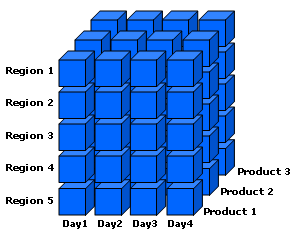
\includegraphics[width=100mm]{img/data-cube.png}
	\caption{An example of~data cube by~Microsoft~\cite{msdn-cube}}
	\label{fig:lod-cloud}
\end{figure}

The Data Cube Vocabulary is~a~concept based on~the~previously mentioned Data Cube and
OLAP cube theory. As~we~are interested in~the~ways of~representing statistical data in~the
Linked Data model, the~reader would not be~surprised, that the~Data Cube 
Vocabulary~\cite{dcv}
concept is~tightly connected to~the~Linked Data model.

Since the~Data Cube Vocabulary is~the~starting point for reaching the~goal of~this thesis,
we will pay a~special attention to~its description. It~combines the~advantages of~the~RDF
model and~Data Cube concept in~order to~make it~easier to~interlink resources involved
in the~published statistics. As~the~Data Cube Vocabulary model is~based on~the~model defined
by Statistical Data and~Metadata eXchange standard~\cite{sdmx}, let us~discuss the~standard a~bit more.

\section{Statistical Data and~Metadata eXchange}
The SDMX Initiative~\cite{sdmx} was introduced by~seven organizations in~order to~make
an~effective standard to~interchange statistical data. All those organizations, e.g. OECD,
UN or~Eurostat, have, without any~doubt, an~access to~a~large amount of~statistical data, even more,
they produce them. Some examples of~such data could be~found on~\cite{pubdata}.
In 2005, the~Initiative has introduced a
version 1.0 of~a~technical specification, which was approved by~the~International
Organization for Standardization~\cite{iso} as~\texttt{ISO:TS 17369}.
Later on, in~May 2011, it~was updated to~version 2.1 (changes in~web services guidelines,
revised data messages, partial code lists and~new metadata management).
In January 2013 the~specification has evolved into~an~International Standard,
\texttt{ISO/IS 17369}~\cite{isosdmx}.

\begin{sloppypar}
The Initiative has also published a~User Guide to~cover major SDMX use cases~\cite{sdmxuserguide}.
It is~focused on~maintaining and~handling statistical data and~its~metadata. It~shows
how to~manage reporting, storage, retrieval and~extending. As~a~natural side--effect,
every organization, which follows the~guide not only solves its~problems with
handling the~data, but is~also able to~interchange those with any~other company
following the~guide.
\end{sloppypar}

That corresponds with the~idea of~the~RDF and~Linked Data models. We~have a~large amount
of datasets we~want to~interchange or~even interlink. Actually, it~comes out of~needs
of the~founding organizations, which cooperate on~the~data they gather. Each of~the~companies creates
a~report, which is~then processed or~often even extended by~one of~the~others. To~make the~chain
of the~data processing more efficient, they agreed on~the~original technical specification.
They focused especially on~the~following issues detected in~the~statistical data exchange:

\begin{itemize}
\item Time consumption of~the~whole processing (data collection, transformations, 
exchange).
\item Different approaches introduced by~different organizations.
\item Different approaches in~how to~utilize new technologies (like XML or~web 
services).
\end{itemize}

While discussing the~standard, several subprojects were introduced. One of~them was to~come
up with a~standardized vocabulary for statistical metadata (metadata common vocabulary). It~was
decided to~use new technologies, such as~web services or~XML, but many of~the~subprojects
were based on~existing concepts, which were utilizing existing technologies. In~the~case of
metadata common vocabulary, it~was \emph{Eurostat’s Concept} and
\emph{Definitions Database (CODED)} and~the~\emph{OECD Glossary of~Terms}.

The important result of~the~process is~\emph{SDMX Content-Oriented Guidelines}.
They were separated
from the~technical specification since they help to~introduce some approaches to~statisticians
for their work. The~technical specification was focused on~developing applications
conforming with the~SDMX model. One could think that it~is~the~technical specification
which enabled us~to~make the~transition between common statistical data and~Linked Data,
but it~were the~SDMX Content--Oriented Guidelines. On~top of~other products, it~introduces the
following:

\begin{itemize}
\item Cross--Domain Concepts.
\item Cross--Domain Codelists.
\item Statistical Subject--Matter Domains.
\item Metadata Common Vocabulary.
\item SDMX--ML for the~Content-Oriented Guidelines (Concepts, Code Lists, Category 
Scheme).
\end{itemize}

These are products that the~Data Cube Vocabulary works with and~builds upon. More important
features were added in~the~revision 2.0. The~SDMX model was extended with reference metadata
concept which tells us~how to~format and~structure metadata with~respect to~data quality
frameworks. Corresponding XML formats were introduced. Furthermore, a~set of~standard XML
interfaces was added to~enable SDMX Registry manipulation. The~registry was introduced to
enable data location catalogization and~metadata cross--referencing over the~Internet. Also,
structured metadata manipulation was introduced.

Since the~SDMX Content--Oriented Guidelines are focused on~SDMX use cases, we~will present
one of~them to~the~reader, since the~same use case could be~applied in~the~derived Data Cube
Vocabulary in~the~environment of~Linked Data.

In fact, the~primary use case designed by~the~Initiative is~called “web data dissemination”
and is~tightly related to~the~Linked Data world. It~comes with a~standardized process of~retrieving
data from the~web periodically and~keeping them up--to--date. It~resembles a~bit a~process
of scraping data into~a~Linked Data datastore, which was, perhaps, derived just from the~web
data dissemination process.

The next SDMX fundamental connected to~the~Linked Data model is~defining concepts. That is
very similar to~the~LD~ontologies. A~concept is~a~source of~data semantics. It:

\begin{itemize}
\item Provides a~detailed definition of~the~component, which describes the~structure of~the~data or
metadata.
\item Can allow data and~metadata for different structures to~be~comparable when~concepts are reused.
\end{itemize}

The goal of~SDMX is~to~reuse existing concepts introduced by~any~community related to~the
given dataset, not to~enforce its own proprietary format. It~is~enforced by~a~rule which states
that a~new concept can be~introduced only if~no~existing concept suffices. The~reason
is that those concepts are already used and~implemented by~a~certain spectrum of
applications, therefore it~will lead to~a~greater interoperability. Similar concepts are then
grouped into~schemes which are versioned. When a~concept changes, a~new version of~the
whole scheme needs to~be~introduced.

\begin{sloppypar}
Also the~list of~three main components of~SDMX concept goes well with~the~Linked Data model
\end{sloppypar}

\begin{itemize}
\item Its identification, which must be~unique within the~scheme.
\item Its name.
\item Its description.
\end{itemize}

One is~also able to~include all those properties into~a~RDF--compliant resource definition,
furthermore, the~first one is~also mandatory and~represented by~a~URI.

\label{SDMX-code-lists}
Hand in~hand with concepts goes defining code lists. It~is~a~way of~determining possible
values. In~fact, those code lists are enumerations. They also have the~three basic components
(identification, name and~description) as~concepts do. Code lists could be~organized into
hierarchies to~reflect a~certain kind of~relations between members of~the~list. The~hierarchy
is meant to~represent a~children--parent relationship, but no~additional properties are specified.
Let us~mention \emph{Nomenclature des Unites Territoriales Statistiques (NUTS)} 
as an~example of~such a~hierarchy.

The data definition reflects exactly what we~need. It~consists of~a~collection of~components, which define what is~being measured together with additional metadata.

\section{Data Cube Vocabulary}
\label{datacube-vocabulary}

\begin{sloppypar}
This model could be~relatively easily decorated with syntactic sugar taken from~the~RDF/LD
world. This is~exactly how the~Data Cube Vocabulary was introduced based
on the~model shown earlier. The~most significant rule of~the~model is~that each
dimension is~needed to~reference a~concept to~determine its semantic meaning.
\end{sloppypar}

But this is~only a~definition of~a~data structure, a~set of~rules of~how a~specific kind of~information
should be~published. Based on~that, a~dataset is~published in~a~way to~respect such a~set
of rules. Therefore, every dataset represents a~collection of~data structures. Each data
structure is~consisted of~a~set of~components. One of~them needs to~be~a~measure,
so--called \emph{primary measure}. The~primary measure is~marked with a~special flag to~be~found
easily to~enable more efficient processing.

Besides measures, there are \emph{dimensions}. A~data structure needs to~have at~least one.
Each dimension references its concept and~has a~unique identification. The~combination of
all the~dimensions (except the~measure) defines a~key, which allows it~to~point
to the~primary measure.

There are some kinds of~specialized dimensions, which can be~defined only once
for a~data structure:

\begin{itemize}
\item Time (point in~time, when the~observation was made).
\item Measure (but could be~a~collection).
\end{itemize}

There are some preferred formats, which tell us~how to~publish the~time of~capturing
the~observation --- a~period, a~duration or~a~timestamp. More details about that could be~found
in the~SDMX User Guide~\cite{sdmxuserguide}.

Moreover, a~data structure can hold some metadata, e.g. the~unit of~the~measurement
or a~starting day of~the~week (in case of~periodic time format).

\begin{sloppypar}
As stated before, the~SDMX 2.0 Information Model was used to~build up~the~RDF
Data Cube Vocabulary, especially the~Content--Oriented Guidelines (COGs). The~Data Cube
vocabulary specification itself does not cover mechanics of~transforming other formats
into the~Data Cube Vocabulary, including the~SDMX mostly used SDMX-ML. It~presents the~final
product, a~model which builds upon the~RDF and~SDMX models.
\end{sloppypar}

In the~section dedicated to~the~brief description of~the~RDF, we~have discussed that resources
are identified by~a~unique identifier --- a~URI. We~have also mentioned that it~is~used to~express
them in~a~compact form while utilizing prefixes and~namespaces. Before going further with
the~description of~the~Data Cube Vocabulary, let us~present a~short list of~significant prefixes
(presented in~the~Table ~\ref{tab:sdmxprefixes}),
since some of~them could appear in~the~text.

\begin{table}[h]\footnotesize
  \caption{Prefixes used frequently with Data Cube Vocabulary}
  \label{tab:sdmxprefixes}
\scriptsize\begin{tabular}{l l~l}
Prefix & Namespace & Brief description \\
\hline
qb & \url{http://purl.org/linked-data/cube#} & Data Cube vocabulary \\
skos & \url{http://www.w3.org/2004/02/skos/core#} & Knowledge Organization Systems dictionary \\
scovo & \url{http://purl.org/NET/scovo#} & Statistical Core Vocabulary \\
void & \url{http://rdfs.org/ns/void#} & Vocabulary of~Interlinked Datasets \\
foaf & \url{http://xmlns.com/foaf/0.1/} & People-related schemes \\
org & \url{http://www.w3.org/ns/org#} & Organizations dictionary \\
dcterms & \url{http://purl.org/dc/terms} & Dublin Core common properties dictionary \\
owl & \url{http://www.w3.org/2002/07/owl#} & Ontologies \\
rdf & \url{http://www.w3.org/1999/02/22-rdf-syntax-ns#} & RDF concepts \\
rdfs & \url{http://www.w3.org/2000/01/rdf-schema#} & RDF schema \\
eg & \url{http://example.org/ns#} & for examples only \\
pc & \url{http://purl.org/procurement/public-contracts#} & Public contracts \\
\end{tabular}\end{table}

The Data Cube Vocabulary reuses the~concept of~a~data structure as~presented in~the~section
dedicated to~the~SDMX description. Therefore, a~data cube is~also consisted of~a~set of
dimensions, attributes and~measures --- components, speaking generally. As~in~the~cases of
OLAP cube and~SDMX, dimensions are used to~uniquely identify observed measures
(remember the~formal mapping marking mentioned in~the~section about RDBMS representation
of OLAP cube). The~outline of~Data Cube Vocabulary can bee seen in~Figure~\ref{fig:lod-cloud}.
 
\begin{figure}
	\centering
	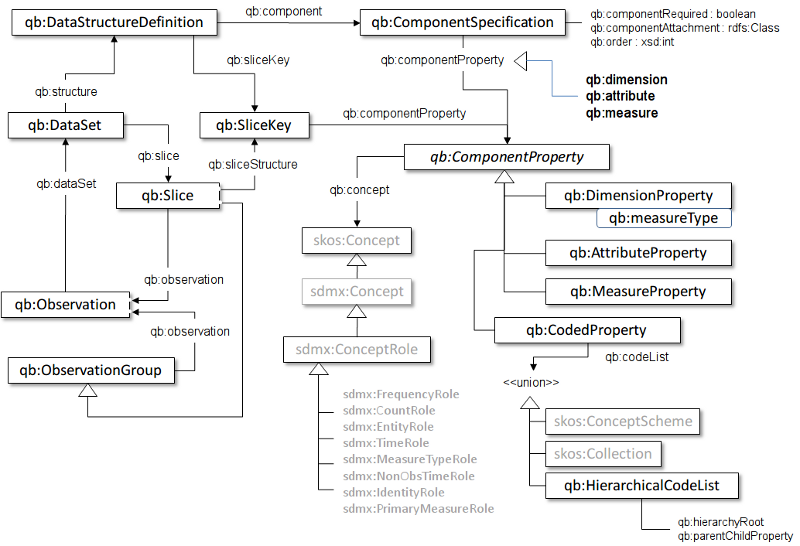
\includegraphics[width=150mm]{img/dcv-schema.png}
	\caption{Data Cube Vocabulary Outline~\cite{dcv}}
	\label{fig:lod-cloud}
\end{figure}

As a~result, we~are perfectly able to~describe the~measurement process - e.g., place, time and
other significant conditions, combined with the~measured value itself. The~whole information
is supplemented with additional attributes, which~may make the~measurement more accurate
- units, multipliers but also other, not so~important, notes.

As we~have discussed in~the~section dedicated to~the~SDMX model, each data set should be
published according to~a~specific data structure. Let us~have a~look on~how the~data structures are
modified by~including Linked Data and~let us~try to~create a~data structure definition according
to our demography example.

A data structure definition is~represented by~\texttt{qb:DataStructureDefinition} resource. It~defines
how the~data set should be~formed in~order to~comply with Data Cube Vocabulary. It~defines
dimensions, attributes and~measures, which may appear in~the~data set. Alongside with the
definition, optional and~required attributes are defined, as~well as~their ordering. This kind
of information can be~extracted easily from a~well--formed document and~needs to~not be~explicitly
declared. But the~explicit declaration enables you to:

\begin{itemize}
\item Verify the~data set structure easily.
\item Determine what dimensions are available for a~given data set.
\item Exchange structure definition.
\end{itemize}

\begin{sloppypar}
Since the~data structure defines attributes, measures and~dimensions, other resources need
to be~involved. That is~why \texttt{qb:ComponentProperty} class was introduced. It~has a~few derived
classes, \texttt{qb:DimensionProperty}, \texttt{qb:AttributeProperty}
and \texttt{qb:MeasureProperty}. Those carry
multiple pieces of~information. Firstly, the~concept, which is~represented (e.g. time, place,
nation, currency, chemical substance, etc.) is~followed by~the~type of~the~component
(dimension, attribute, measure). Last but not least, it~carries the~information about which
code list (see section~\ref{SDMX-code-lists}) is~used to~represent the~value.
\end{sloppypar}

Since the~goal of~the~SDMX model and~Data Cube Vocabulary is~to~reuse community--proposed
taxonomies, \texttt{qb:concept} property was introduced to~make it~possible to~link
\texttt{qb:ComponentProperty} with an~existing concept. \emph{SKOS vocabulary} is~used to
represent such concepts. SKOS does not define any~specific concepts. It~just defines
a~vocabulary for concept interlinking.

\begin{sloppypar}
One could specify the~range of~the~concept while defining a~value of~the~\texttt{rdfs:range} property.
Also, the~concepts may be~used repeatedly in~a~data set in~different roles.
For example, time could be~used as~a~dimension (in the~meaning that something was measured
in the~year 2012) as~well as~a~measured value (something took 203 seconds).
\end{sloppypar}

It is~of~a~great help, if~the~value is~a~part of~an~enumeration defined in~a~code list. Due to
the~existence of~the~qb:codeList property, an~automatic validation and~range checking
can be~performed. Moreover, tools can easily retrieve the~complete list of~possible values.
To enable range checking on~non--coded values, rdfs:range can be~used.

\begin{sloppypar}
Before getting back to~our example, we~need to~point out a~bridge between the~SDMX
and Data Cube Vocabulary models. A~community group has introduced some RDF 
encodings of~SDMX COGs. These are \texttt{sdmx-concept}, \texttt{sdmx-code}, \texttt{sdmx-dimension},
\texttt{sdmx-attribute} and~\texttt{sdmx-measure}. That is~a~simple way of~interlinking the~Data Cube
Vocabulary with the~SDMX model.
\end{sloppypar}

Let us~get back to~the~demography example. We~will continue with the~prepared RDF
document and~transform it~into~a~Data Cube Vocabulary model. Since we~know that each
observation should conform to~a~specified data structure, we~should at~first define
such a~structure. To~define a~structure, we~need to~define all components first.
We will use slightly modified examples presented in~the~Data Cube vocabulary
definition since it~fits our use case:

\begin{enumerate}
\item Time definition [dimension]:

\begin{verbatim}
eg:refPeriod a rdf:Property, qb:DimensionProperty ;
    rdfs:label "reference period"@en ;
    rdfs:subPropertyOf sdmx-dimension:refPeriod ;
    rdfs:range interval:Interval ;
    qb:concept sdmx-concept:refPeriod .
\end{verbatim}

We define the~\texttt{eg:refPeriod} and~we~state, that it~is~a~\texttt{rdf:Property} and~Data Cube dimension.
The rest of~the~statements are metadata, which~are not really necessary, textual description
(label) and~interlinking with existing concepts (relations to~sdmx-dimension). To~enable range
cheking, \texttt{rdfs:range} is~defined.

\item Place definiton [dimension]:

\begin{verbatim}
eg:refArea a rdf:Property, qb:DimensionProperty ;
    rdfs:label "reference area"@en ;
    rdfs:subPropertyOf sdmx-dimension:refArea ;
    rdfs:range admingeo:UnitaryAuthority ;
    qb:concept sdmx-concept:refArea .
\end{verbatim}

\item Population count definiton [measure]:
\begin{verbatim}
eg:finalPopulation a rdf:Property, qb:MeasureProperty ;
      rdfs:label "the total number of citizens"@en ;
      rdfs:subPropertyOf sdmx-measure:obsValue ;
      rdfs:range xsd:decimal .
\end{verbatim}
\end{enumerate}

\begin{sloppypar}
It is~important to~notice the~link to~the~\texttt{sdmx-measure:obsValue}, which~is~the~special flag
mentioned in~the~section dedicated to~description of~SDMX values. With the~power of~SPARQL
it is~very easy to~query a~triple store for~all the~values, which are the~observation values to~get
all values in~a~given graph. In~fact, it~should be~sufficient to~query all instances of
\texttt{qb:MeasureProperty}, the~relation to~\texttt{sdmx-measure:obsValue} just makes the~definition
more precise. An~example of~such a~SPARQL query can be~seen in~Figure~\ref{fig:sparql-obsValue}.
\end{sloppypar}

\begin{figure}
\begin{verbatim}
  
  SELECT ?v WHERE {
    ?v a ?x .
    ?x rdfs:subPropertyOf sdmx-measure:obsValue .
  }

\end{verbatim}
\caption{A SPARQL query, which retrieves all observation values from a~dataset}
\label{fig:sparql-obsValue}
\end{figure}

It is~natural that while performing a~measurement, you can retrieve multiple
values within a~single observation. A~good example of~such an~observation could be~weather
information sampling. One can measure many physical values (e.g. temperature, air pressure,
humidity, …) in~a~specific timeframe on~a~specific place. One can store those values separately,
each in~a~standalone observation. But since the~observation has been made at~the~same moment
and the~dimensions are exactly the~same, it~is~only natural to~add those value components
into~the~same observation. One will end up~with a~5--dimensional observation where 2 components 
are dimension properties (place and~time) and~3 components are measure properties
(temperature, pressure, humidity). Without grouping, one would make 3 related observations,
each with a~single measure property (3 dimensions overall).

Regardless of~whether you group those observations into~a~single one or~not, one is~able
to select the~related observations from the~data cube dataset relatively easily since they
are all determined by~exactly the~same dimension properties. That is~called \emph{slicing}.
If you take a~cube and~select all the~related observations you make a~slice. The~slice is~exactly
the~same as~the~5--dimensional observation mentioned before.

Based on~the~data structure, we~can publish a~specific dataset. The~dataset could be~formalized
as a~collection of~four data types:
\begin{sloppypar}
\begin{itemize}
\item Observations --- values, measured numbers.
\item Organizational structure --- dimensions of~the~measured value (could be~in~the~form of~slices)
\item Internal metadata --- additional data description used to~interpret observations (units, estimation,
etc.).
\item External metadata --- interlink to~an~author, dataset categorization, etc. (linked data 
principle).
\end{itemize}
\end{sloppypar}

An example of~such a~dataset can be~seen in~Figure~\ref{fig:example-dcv-dataset}.

\begin{figure}
\tiny\begin{verbatim}
@prefix rdf:     <http://www.w3.org/1999/02/22-rdf-syntax-ns#> .
@prefix rdfs:    <http://www.w3.org/2000/01/rdf-schema#> .
@prefix owl:     <http://www.w3.org/2002/07/owl#> .
@prefix skos:    <http://www.w3.org/2004/02/skos/core#> .
@prefix foaf:    <http://xmlns.com/foaf/0.1/> .
@prefix scovo:   <http://purl.org/NET/scovo#> .
@prefix void:    <http://rdfs.org/ns/void#> .
@prefix vcard:   <http://www.w3.org/2006/vcard/ns#> .
@prefix xsd:     <http://www.w3.org/2001/XMLSchema#> .
@prefix dcterms: <http://purl.org/dc/terms/>.

@prefix qb:              <http://purl.org/linked-data/cube#> .
@prefix sdmx:            <http://purl.org/linked-data/sdmx#> .
@prefix sdmx-concept:    <http://purl.org/linked-data/sdmx/2009/concept#> .
@prefix sdmx-dimension:  <http://purl.org/linked-data/sdmx/2009/dimension#> .
@prefix sdmx-attribute:  <http://purl.org/linked-data/sdmx/2009/attribute#> .
@prefix sdmx-measure:    <http://purl.org/linked-data/sdmx/2009/measure#> .
@prefix sdmx-metadata:   <http://purl.org/linked-data/sdmx/2009/metadata#> .
@prefix sdmx-code:       <http://purl.org/linked-data/sdmx/2009/code#> .
@prefix sdmx-subject:    <http://purl.org/linked-data/sdmx/2009/subject#> .

@prefix eugeo: <http://ec.europa.eu/eurostat/ramon/ontologies/geographic.rdf#> .

@prefix czso-teritorries:  <http://purl.org/cszo/teritorries#> .
@prefix czso-ds-dem-pop:   <http://linked.opendata.cz/resource/czso.cz/dataset/demography/final-population#> .
@prefix czso-ds-dem-bir:   <http://linked.opendata.cz/resource/czso.cz/dataset/demography/births#> .
@prefix czso-ds-dem-dea:   <http://linked.opendata.cz/resource/czso.cz/dataset/demography/deaths#> .
@prefix czso-ds-dem-imm:   <http://linked.opendata.cz/resource/czso.cz/dataset/demography/immigrants#> .
@prefix czso-ds-dem-emm:   <http://linked.opendata.cz/resource/czso.cz/dataset/demography/emmigrants#> .
@prefix czso-ds-def:       <http://linked.opendata.cz/resource/czso.cz/dataset-definitions#> .

czso-ds-dem-pop: a sdmx:DataSet ;
  dcterms:subject <http://eulersharp.sourceforge.net/2003/03swap/countries#cz>, <http://dbpedia.org/resource/Czech_Republic> ;
  dcterms:publisher <http://opendata.cz/me#> ;
  sdmx:maintainer <http://linked.opendata.cz/resource/business-entity/00025593> ;
  dcterms:date "2012-09-05"^^xsd:date ;
  qb:structure czso-ds-def:DemographyFinalPopulationDefinition .
  
czso-ds-dem-bir: a sdmx:DataSet ;
  dcterms:subject <http://eulersharp.sourceforge.net/2003/03swap/countries#cz>, <http://dbpedia.org/resource/Czech_Republic> ;
  dcterms:publisher <http://opendata.cz/me#> ;
  sdmx:maintainer <http://linked.opendata.cz/resource/business-entity/00025593> ;
  dcterms:date "2012-09-05"^^xsd:date ;
  qb:structure czso-ds-def:DemographyBirthsDefinition .
  
czso-ds-dem-dea: a sdmx:DataSet ;
  dcterms:subject <http://eulersharp.sourceforge.net/2003/03swap/countries#cz>, <http://dbpedia.org/resource/Czech_Republic> ;
  dcterms:publisher <http://opendata.cz/me#> ;
  sdmx:maintainer <http://linked.opendata.cz/resource/business-entity/00025593> ;
  dcterms:date "2012-09-05"^^xsd:date ;
  qb:structure czso-ds-def:DemographyDeathsDefinition .
  
czso-ds-dem-imm: a sdmx:DataSet ;
  dcterms:subject <http://eulersharp.sourceforge.net/2003/03swap/countries#cz>, <http://dbpedia.org/resource/Czech_Republic> ;
  dcterms:publisher <http://opendata.cz/me#> ;
  sdmx:maintainer <http://linked.opendata.cz/resource/business-entity/00025593> ;
  dcterms:date "2012-09-05"^^xsd:date ;
  qb:structure czso-ds-def:DemographyImmigrantsDefinition .
  
czso-ds-dem-emm: a sdmx:DataSet ;
  dcterms:subject <http://eulersharp.sourceforge.net/2003/03swap/countries#cz>, <http://dbpedia.org/resource/Czech_Republic> ;
  dcterms:publisher <http://opendata.cz/me#> ;
  sdmx:maintainer <http://linked.opendata.cz/resource/business-entity/00025593> ;
  dcterms:date "2012-09-05"^^xsd:date ;
  qb:structure czso-ds-def:DemographyEmmigrantsDefinition .
  
<http://linked.opendata.cz/resource/czso.cz/dataset/demography/final-population/554782-2011> a qb:Observation ;
    qb:dataSet <http://linked.opendata.cz/resource/czso.cz/dataset/demography/final-population#> ;
    czso-ds-def:refArea <http://linked.opendata.cz/resource/region/554782> ;
    czso-ds-def:refPeriod "2011"^^xsd:gYear ;
    czso-ds-def:finalPopulation "1241664"^^xsd:nonNegativeInteger .

<http://linked.opendata.cz/resource/czso.cz/dataset/demography/births/554782-2011> a qb:Observation ;
    qb:dataSet <http://linked.opendata.cz/resource/czso.cz/dataset/demography/births#> ;
    czso-ds-def:refArea <http://linked.opendata.cz/resource/region/554782> ;
    czso-ds-def:refPeriod "2011"^^xsd:gYear ;
    czso-ds-def:births "13968"^^xsd:nonNegativeInteger .
\end{verbatim}\normalsize
\caption{An example of~a~DCV dataset by~OpenData.cz}
\label{fig:example-dcv-dataset}
\end{figure}

In this chapter, we~have introduced a~long process of~transforming a~simple statement into
a~form, which is~compliant with the~Data Cube Vocabulary standard. The~original statement
was processed while applying a~set of~a~simple transformation steps, at~least from the~point of~view
of a~human brain. The~goal of~this thesis is~to~make one of~these steps as~automatic as~possible 
in order to~come up~with a~prototype of~a~system, which is~able to~transform an~arbitrary set of~RDF data
into a~Data Cube Vocabulary form, if~possible. Also, a~user input (a set of~transformation rules) is
needed to~get such a~task done. 

\begin{sloppypar}
Since Payola was designed to~provide a~platform for analyzing and~visualizing 
Linked Data and~its main goal is~to~lower the~knowledge barrier, which~one
needs to~overcome in~order to~analyze Linked Data, we~also want all the~newly--introduced 
components to~fit into~the~concept of~the~whole platform --- to~be~reusable.
We~will also demonstrate the~benefits of~such transformations while implementing 
a~visualization, which will take advantage of~the~Data Cube Vocabulary.
\end{sloppypar}
